
\begin{tikzpicture}
    \node[draw, label={$\tau_1$}, thick] (T_A) at(0,0) {
        \begin{tikzpicture}
            \node[circle, draw, thick, inner sep=0pt, minimum width=1cm] (t1) at (0,0) {$\tau_1^1$};
            \node[circle, draw, thick, inner sep=0pt, minimum width=1cm] (t2) at (-0.7,-1.4) {$\tau_1^2$};
            \node[circle, draw, thick, inner sep=0pt, minimum width=1cm] (t3) at (0.7,-1.4) {$\tau_1^3$};
            \node[circle, draw, thick, inner sep=0pt, minimum width=1cm] (t4) at (0,-2.8) {$\tau_1^4$};
            \draw[>=latex,thick,->] (t1)--(t2);
            \draw[>=latex,thick,->] (t1)--(t3);
            \draw[>=latex,thick,->] (t2)--(t4);
            \draw[>=latex,thick,->] (t3)--(t4);
        \end{tikzpicture}
    };
    \node[draw, label={$\tau_2$}, thick] (T_B) at (3.5,0) {
        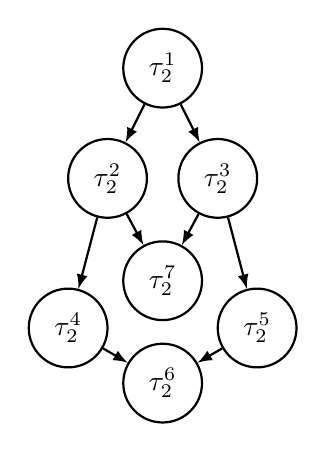
\begin{tikzpicture}
            % SEQ 1
            \node[circle, draw, thick, inner sep=0pt, minimum width=1cm] (t5) at (0,0) {$\tau_2^1$};
            \node[circle, draw, thick, inner sep=0pt, minimum width=1cm] (t6) at (-0.7,-1.4) {$\tau_2^2$};
            \node[circle, draw, thick, inner sep=0pt, minimum width=1cm] (t7) at (0.7,-1.4) {$\tau_2^3$};
            % SEQ 2
                \node[circle, draw, thick, inner sep=0pt, minimum width=1cm] (t8) at (-1.2,-3.3) {$\tau_2^4$};
            \node[circle, draw, thick, inner sep=0pt, minimum width=1cm] (t9) at (1.2,-3.3) {$\tau_2^5$};
            \node[circle, draw, thick, inner sep=0pt, minimum width=1cm] (t10) at (0,-4) {$\tau_2^6$};
            % SEQ 3
            \node[circle, draw, thick, inner sep=0pt, minimum width=1cm] (t11) at (0,-2.7) {$\tau_2^7$};
    
            % SEQ 1
            \draw[>=latex, thick,->] (t5)--(t6);
            \draw[>=latex, thick,->] (t5)--(t7);
            % SEQ 2
            \draw[>=latex, thick,->] (t8)--(t10);
            \draw[>=latex, thick,->] (t9)--(t10);
    
            % SEQ 1 -> SEQ 2
            \draw[>=latex, thick,->] (t6)--(t8);
            \draw[>=latex, thick,->] (t7)--(t9);
            % SEQ 1 -> SEQ 3
            \draw[>=latex, thick,->] (t6)--(t11);
            \draw[>=latex, thick,->] (t7)--(t11);
        \end{tikzpicture}
    };
\end{tikzpicture}
